\documentclass{article}
\usepackage[utf8]{inputenc}
\usepackage[nottoc]{tocbibind}
\usepackage[english]{babel}
\usepackage{graphicx}
\setlength{\parindent}{0pt}
\setlength{\parskip}{1ex plus 0.5ex minus 0.2ex}
\usepackage{float}
\usepackage{wrapfig}
\usepackage{caption} 
\usepackage{subcaption}
\usepackage{capt-of}
\usepackage{color}
\usepackage{enumerate}
\usepackage{amsmath}
\usepackage{setspace}
\usepackage{biblatex}
\addbibresource{References.bib}
\usepackage[utf8]{inputenc}
\usepackage[T1]{fontenc}
\usepackage{comment}
\usepackage{subcaption}
\usepackage{geometry}
\usepackage[final]{pdfpages}
% \usepackage[backend=bibtex]{biblatex}



% til R input

\usepackage[svgnames]{xcolor}
\usepackage{listings}

\lstset{language=R,
    basicstyle=\small\ttfamily,
    stringstyle=\color{DarkGreen},
    otherkeywords={0,1,2,3,4,5,6,7,8,9},
    morekeywords={TRUE,FALSE},
    deletekeywords={data,frame,length,as,character},
    keywordstyle=\color{blue},
    commentstyle=\color{DarkGreen},
}

\definecolor{mygreen}{RGB}{28,172,0}
\definecolor{mylilas}{RGB}{170,55,241}




% hyperref
\usepackage{hyperref}
\hypersetup{
    colorlinks=true,
    citecolor=black,
    urlcolor=blue,
    linkcolor=black
}

\usepackage{color}
\usepackage{siunitx}
\sisetup{output-decimal-marker={,}}


%header and footer
\usepackage{fancyhdr}
\pagestyle{fancy}
\lhead{
Master thesis}
\chead{}
\rhead{Kia Kafaei}
\lfoot{}
\cfoot{}
\usepackage{lastpage}
\rfoot{\thepage\ af \pageref{LastPage}}

\title{}
\author{}
\date{}


\begin{document}
\large

\begin{titlepage}

%\begin{flushright}
%
\includegraphics[width=30mm]{billeder/dtulogo.png}
%\end{flushright}

\begin{center}
    
\vspace{10mm}
\noindent {\LARGE \textbf{ Master Thesis}}
\vspace{5mm}\\


\begin{figure}[t]
    \vspace*{-1cm}
    \hspace{14 cm}
    
\includegraphics[scale=0.1]{fig/dtulogo.png}
\end{figure}

\noindent { \large \textbf{
}}

\noindent { \large \textbf{Technical University of Denmark}}
%\line(1,0){\textwidth}

\vspace{5mm}

Navigerbarhed med BIM modeller

\noindent { \large \textbf{\today}}

% \vspace{15mm}
% \noindent {\large \textbf{\underline{\textbf{GROUP 14}}}}

\vspace{5mm}
Kia Kafaei Yahyavi

\end{center}

\vspace{29mm}

% \begin{figure}[H]
%     \hspace*{-2.7cm}
%     \includegraphics[scale = 0.9]{DTUBanner.png}
%     \vspace*{-0.1 cm}
% \end{figure}

\end{titlepage}




%\section{Different sections to write about}

\subsection{Previous work}
\begin{itemize}
    \item Write about the 3 week project Gwayfinding
\end{itemize}

\subsection{Litteratur review}
\begin{itemize}
    \item Write about the paper that explains people pathfinding in building, where they use grid instead of polygonal
    \item Write about pathfinding in 2d world master thesis. How they describe the difference between polygonal and grid, what algorithms to use for each etc.
    \item Write about the TSP problem, and its solutions. Find paper for that perhaps.
    \item Maybe find paper about Spot.
\end{itemize}


\subsection{Plotting floorplans}
\begin{itemize}
    \item Section about preprocessing of the dataset
    \item Section about the data and the polygonal triangle structure of the dataset, and why it makes sense.
    \item Talk about removing redundant lines from triangles.
    \item Talk about the challenges of plotting the doors. How I did this manually instead.
\end{itemize}

\subsection{Grid vs polygonal}
\begin{itemize}
    \item Talk about how you could use the grid version or the polygonal version. Spent a good amount of effort here.
\end{itemize}

\subsection{Which platform to use}
\begin{itemize}
    \item Write about which platform to use. The pros and cons of each. Ros vs Unity vs Python.
\end{itemize}


\subsection{TSP}
\begin{itemize}
    \item How to represent nodes and graphs? Comparison of different ways and libraries
    \item Making a weighted graph of all the nodes, where the weights are the Euclidean distance between each node. Write that it is a undirected graph.
    \item A section on the line intersection algorithm used for connecting the points
    \item Using dijkstra's/A* to make a complete subgraph of all the relevant nodes, and how this problem is a bit different than the traditional tsp.
    \item A section of the 2-OPT algorithm and how it uses Minimum Spanning Tree and a DFS traversal. You can talk about alternative algorithms and ther pros and cons.
    \item A section describing the MST and DFS algorithms and how Networkx implementation work. Maybe a section about adjacency list vs matrix, kruskal vs prims. When to use which.
\end{itemize}

\subsection{Dimensions of robot}
\begin{itemize}
    \item Write about how to incorporate the dimensions of the robot in your simulation
\end{itemize}

\subsection{Optimal placement of nodes}
\begin{itemize}
    \item Write about scenic route vs discrete points.
    \item Write about SLAM
    \item optimal placement of nodes
\end{itemize}

\subsection{Spot}
\begin{itemize}
    \item Write about Spot and how it is a usefull robot for this thesis
    \item Write about different platforms for programming Spot, python API vs ROS.
\end{itemize}

\subsection{Future work}
\begin{itemize}
    \item A section about stairs
\end{itemize}
%\section{Introduction}

\section*{Motivation}
Why is it interesting?
The project is being worked on in collaboration with Dalux which is a software company that makes BIM models (Building information modelling). At the moment Dalux has to hire an expensive arcitect to walk around the construction site to check up on that everything is going according to plan and that there aren’t any errors. If this process could be automated such that a robot could walk around a construction instead and send the data directly to Dalux’ software, that would be of great benefit for Dalux. 


\section{Abstract}
Første problem. En bim model ind og finde fra a til b.
\begin{itemize}
    \item Make a simulation of a particle moving from one point to another
    \item Make the simulation include walls and obstacles
    \item Transfer walls from a real BIM model onto simulation
    \item Make a maximum coverage algorithm to find specific nodes that are most optimal for point clouds
    \item Find an optimal route for the particle to move between maximum coverage nodes.
    \item Start testing on the robot and include 
\end{itemize}



\section*{Objective}
The objective of this project is to program the spot robot from Boston Dynamics
to move around construction sites. The robot should be able to walk around the entire construction site on its own and should – while walking – take pictures (or/and point scans) of the construction site. The purpose of this is that after the construction workers have done their day of work the spot robot should wake up at night and walk around the construction site to see if everything is going according to plan and if all deadlines and milestones are met.

What should be done?
Boundaries: what can I probably not do?
Risk analysis: What parts of the project are going to be difficult



\section*{Previous work}

\section*{Introduction}
Explain what you’re going to do

\section*{Literature review}
(Write about what the field around your research looks like)

\section*{Dataset}
Describe your dataset(s), including literature relevant to that dataset, if any

\section*{Results}
(Tell us what you have found)

\section*{Conclusion}
(Summarize your findings, bring in perspectives)
Notes on what works and didn’t work:

\section*{Litteratur list}


\section{Svar på spm}
\subsection{Skal jeg skrive i passiv eller aktiv form?}
The project is being worked on in collaboration with...
I am working on the project in collaboration with…
\\\\
Brug aktiv form. En gang på siden bruge “I”.
Som regel inkluderer man læseren og bruger “We”, hvis det er noget du har lavet så “I”.
Tit bruger man ikke personer som subjekt.
Brug mest aktiv, der må gerne være lidt passivt.


Gulv areal hvert pixel bliver et grid punk. Skyd en email hvis du løbetr ind i problemer.
Unity reflect det der oversætter bim modeller til unity. Hen ad vejen måske.
Ray trace bim model der kunen hjælpe med at finde ud af fra et punkt til et andet.



%\section{Previous work}
\subsection{Wayfinding}
In the paper Wayfinding (insert reference) which is a DTU project in collaboration with Dalux, the goal was to do a pathfinding for a worker in a building. This is similar to what will be done in this thesis and therefore a lot of the same groundwork is done. The dataset is also the same, which makes it easy to translate the results and compare. Even though there was no access to the source code they used to generate their algorithms the report gave good inspiration to what should be done and it also worked as a guide for me to get started. I will be using this report as a reference thorughout this thesis.


\section{Teori områder}

\begin{itemize}
    \item BIM
    \item Graph teori.
    \item kinematic 
    \item Pathfinding A*
    \item Start med minimum spanning tree med kruskals algorithm: https://www.youtube.com/watch?v=Rc6SIG2Q4y0
    \item TSP problem:
https://www.youtube.com/watch?v=M5UggIrAOME
    \item Dernæst tjek chrisofides/ prims algoritm
\end{itemize}




\subsection{Dataset}
The dataset consists of html code of the room coordinates and the door coordinates. The coordinates are givin in a polygonal triangle structure. This means that the floorplan is drawn from these coordinates by a mesh of triangle polygonals. Each room from in the floorplan consists of its own tree branch, which makes it easy to include or exclude rooms in the floorplan. 
Describing rooms and floorplans with triangle forming coordinates is a common way and makes sense for many reasons.
(Insert article reference that describes this way of plotting rooms)

There are also alternative ways to do this. 
(Insert article reference that describes alternative ways to do this)


(Insert picture of floorplan with triangles).
\\
The door coordinates also consists of the set of 3 coordinates with a x,y and z coordinate. Where the z coordinate says how tall the door is. 
\\
BIM models is also available for use, but will not necessarily be used since we start by modelling in 2D.
(Describe BIM models)

\subsection{Plotting floorplans}
\subsubsection{Preprocessing of the dataset}
Before working with the dataset some preprocessing had to be done. This included splitting the array values in appropriate ways and gathering them in sets of three such that the triangles could be formed. The coordinate\_processing module that I made took care of this.

\subsubsection{Removing redundant lines}
The triangle structure of the dataset forms a mesh that spans the entire floorplan. This does not do a great job of visualising the floorplan in an appropriate way. Some preprocessing has to be done to make the rooms in the floorplan distinguishable from eachother. With a bit of intutition it can be seen that the lines to be removed are a part of more than one triangle, if e.g two triangles are used to span a room the line that should be removed is the one shared by both triangles. The way to remove the redundant lines is by using hashing. The idea here is to make a dictionary where each line is given a key and the same lines will have the same key. The way to make sure that the same lines will get the same key is by using hashing. Then all keys with more than one value (line) will be removed. The idea of using hashing to remove redundant lines was taken from this project (insert project reference).

\subsubsection{Plotting the doors}
When plotting the doors a challenge occured, which was that a transformation had to be performed on the doors before they were aligned with the rest of the floorplan. 
This was due to the way the dataset was gathered and the reason for this is unknown. 
Therefore the doors would have to be placed manually before further analysis could happen.



\subsection{Grid vs polygonal}

Talk about how you could use the grid version or the polygonal version. Spent a good amount of effort here.

\subsection{Which platform to use}
\begin{itemize}
    \item Write about which platform to use. The pros and cons of each. Ros vs Unity vs Python.
\end{itemize}



\subsection{TSP}
\begin{itemize}
    \item How to represent nodes and graphs? Comparison of different ways and libraries
    \item Making a weighted graph of all the nodes, where the weights are the Euclidean distance between each node. Write that it is a undirected graph.
    \item A section on the line intersection algorithm used for connecting the points
    \item Using dijkstra's/A* to make a complete subgraph of all the relevant nodes, and how this problem is a bit different than the traditional tsp.
    \item A section of the 2-OPT algorithm and how it uses Minimum Spanning Tree and a DFS traversal. You can talk about alternative algorithms and ther pros and cons.
    \item A section describing the MST and DFS algorithms and how Networkx implementation work. Maybe a section about adjacency list vs matrix, kruskal vs prims. When to use which.
\end{itemize}

\subsubsection{Line intersection}
When determining whether to points on a map are traversable some sort of line intersection algorithm is used. Without using
line intersection the program wouldn't be able to detect whether there are walls between two points, and it would therefore always
choose the shortest distance between two points to be a straight line, regardless if it passes through walls or not. 

(insert reference https://bryceboe.com/2006/10/23/line-segment-intersection-algorithm/)

The algorithm chosen in this case works by checking first if three points are counterclockwise of eachother.




\subsection{Dijkstra's algorithm}
Dijkstra's algorithm is an algorithm to find the shortest path between two nodes in graph. The way it works is by first having a source node or initial node. The distances to all other nodes will be initialized to infinity since the distances are unknown for now. Then the algorithm will look at the neighboor nodes of the source node. It will evaluate the distance to each of the nodes. The distances of the nodes will then be updated in the table of distances, since it is no longer infinity. With done the start node has been visited and will no longer be visited. The next node in the algortihm to evaluate will be the node with the shortest distance to the start node. The neighboors to this node will now be evaluated and again the distance table will be updated. This pattern will keep repeating untill all nodes have been evaluated. 

\subsection{A*}
A

\subsection{How to get around the building}
The way to get around the building is using visibility graph. Here you make a node on each portruding corner and also on the doors. This way a path between all nodes can be constructed, this is called a visibility graph.
(reference the master thesis).

\subsection{How to get from room to room/around the building in a appropriate way?}
Do we want the shortest route?
Do we want the route



\subsection{Dimensions of robot}
\begin{itemize}
    \item Write about how to incorporate the dimensions of the robot in your simulation
\end{itemize}


\subsubsection{Distance field vs distance route}
The dimensions of the robot is mostly needed to make sure that the robot does not bump into walls or other objects. And also to make sure that a path that is deemed traversable is not in reality too narrow for the robot to pass through.
So far the robot has been modeled by a point, it is now time to include a radius to that point which will represent the robots dimensions.

There are multiple ways to go about the challenge of incorporating the dimensions of the robot in the simulation. 
One way is to discretize the entire map and for each cell find the distance to the nearest wall. If the distance from the wall to the cell is smaller than the radius of the robot, the cell will be deemed not traversable since this means that the robot will hit the wall. If the distance to the wall is larger than the radius the cell is traversable. What we get by doing this is a boolean distance field. Where we have nodes that are traversable and nodes that aren't.
The issue with this approach is that it is not very scalable to bigger buildings. More on this is written in chapter 10.
The good thing about this approach is that it is easy and a straightforward way to tell the robot which places it is allowed to traverse and which are not. It can not go wrong with this approach. 
It is also fast to look up because you have done the preprocessing before hand.


The other way is to discretize the route. This is a bit more complicated implementation but will be rewarded by its scalability to bigger buildings. 
The idea here is to only discretize the route that the robot will walking instead of discretizing the entire map. 
Along the route the robot will check if it is near a wall using a distance function. The interval here can be dynamic e.g if the distance to the nearest wall is 5 meters and the radius of the robot is 1 meter it can walk for 4 meter without hitting a wall.
This means that between 2 nodes - a start and an end node - a lot more nodes will be placed. The robot will go to a node find the distance to the nearest wall and then check walk in a straight line towards the node it is seeking the same amount as the distance to the nearest wall minus the radius. Then it will check again to see what the distance to the nearest wall is and repeat the process. It is important that the room/end nodes are a certain radius away from the walls to begin with. 

One way to go about this is to check the distance to all the walls for every node. This does not scale very well when the number of walls increases. 
Another way is to have a certain datastructure that takes all the walls and find the nearest quickly.





















\subsection{Optimal placement of nodes}
\begin{itemize}
    \item Write about scenic route vs discrete points.
    \item Write about SLAM
    \item optimal placement of nodes
\end{itemize}

\subsubsection{Simultanous location and mapping}
As the name indicates SLAM is about localizing your robot in the map while you also do the mapping part. The way this is done is by using sensors such as a lidar - it could also be other types of sensors. Then there are some other steps in the process. Since inn this case the mapping has already been done it doesn't really make sense to do the SLAM. It might be a good idea to find a way for the robot to localize itself, without need to do the mapping.



\subsection{Spot}
\begin{itemize}
    \item Write about Spot and how it is a usefull robot for this thesis
    \item Write about different platforms for programming Spot, python API vs ROS.
\end{itemize}

\subsection{Future work}
\begin{itemize}
    \item A section about stairs
\end{itemize}



% \section*{Methods}
Describe the tools you’ve used

\subsection{My process}
\begin{itemize}
    \item I spent a week or 2 to create the floor plan in python. I then got stuck with the doors since they do not match in any sort of way.
    \item I moved on to experimenting with unity. Making a grid system that could implement A*.
    \item I spent time researching whether to use the grid system or the graph/polygonal system.
    \item I went back to trying to find the best software for simulation in the future also.
    \item Now I am back to implementing the algorithm in python 2D like they did in the 3 week report, before doing the simulation in unity.
    \item I implemented the TSP solution to the problem. 
    \item I visited the Spot robot in Odense
\end{itemize}


\subsection{General questions to answer}
\begin{itemize}
    \item How to get around the building
    \item How to get from room to room/around the building in an appropriate way?
\end{itemize}


%\section*{Discussion}
(Comment on your results, explain what those results mean, interpret the results in a wider context. Also indicate which results were expected or unexpected, and provide an explanation for the unexpected results)


\subsection{Grid vs graph connectivity}
Explain
\begin{itemize}
    \item both methods 
    \item that the graph doesn't work on weird buildings but grid system does.
    \item That grid scales badly with building size but graph doesn't
    \item f
    \item f
    \item f
    \item Maybe variation in node sizes help
    \item That the robot needs a certain node size to work properly. It doesn't work on nodes in the $mm^2$ range.
\end{itemize}


To make the robot walk from one room to another or one place in the building to another, it is important to understand the and decide on a way to implement the connectivity between the rooms. There are mainly two different kinds of implementations; a graph connectivity implementation and a grid implementation.
\\\\
The grid implementation works by discretizing the floor of the building into a grid with nodes of a specific size; the smaller the node size the higher the resolution of the grid.
\\
The graph connectivity approach works by representing each room/area by a node/dot which will be connected by a line to other rooms in the floor.

The different implementations have different advantages and limitations. For example computationally the graph connectivity approach is much more scalable with bigger buildings or construction sites where as implementing a grid system in these situations will be more taxing computationally since a lot of nodes will have to be calculated. 

On the other hand the advantage of the grid method is that its pathfinding algorithms will work on all building shapes. 
Imagine the floor plan of the building below:


\begin{figure}[H]
    \centering
    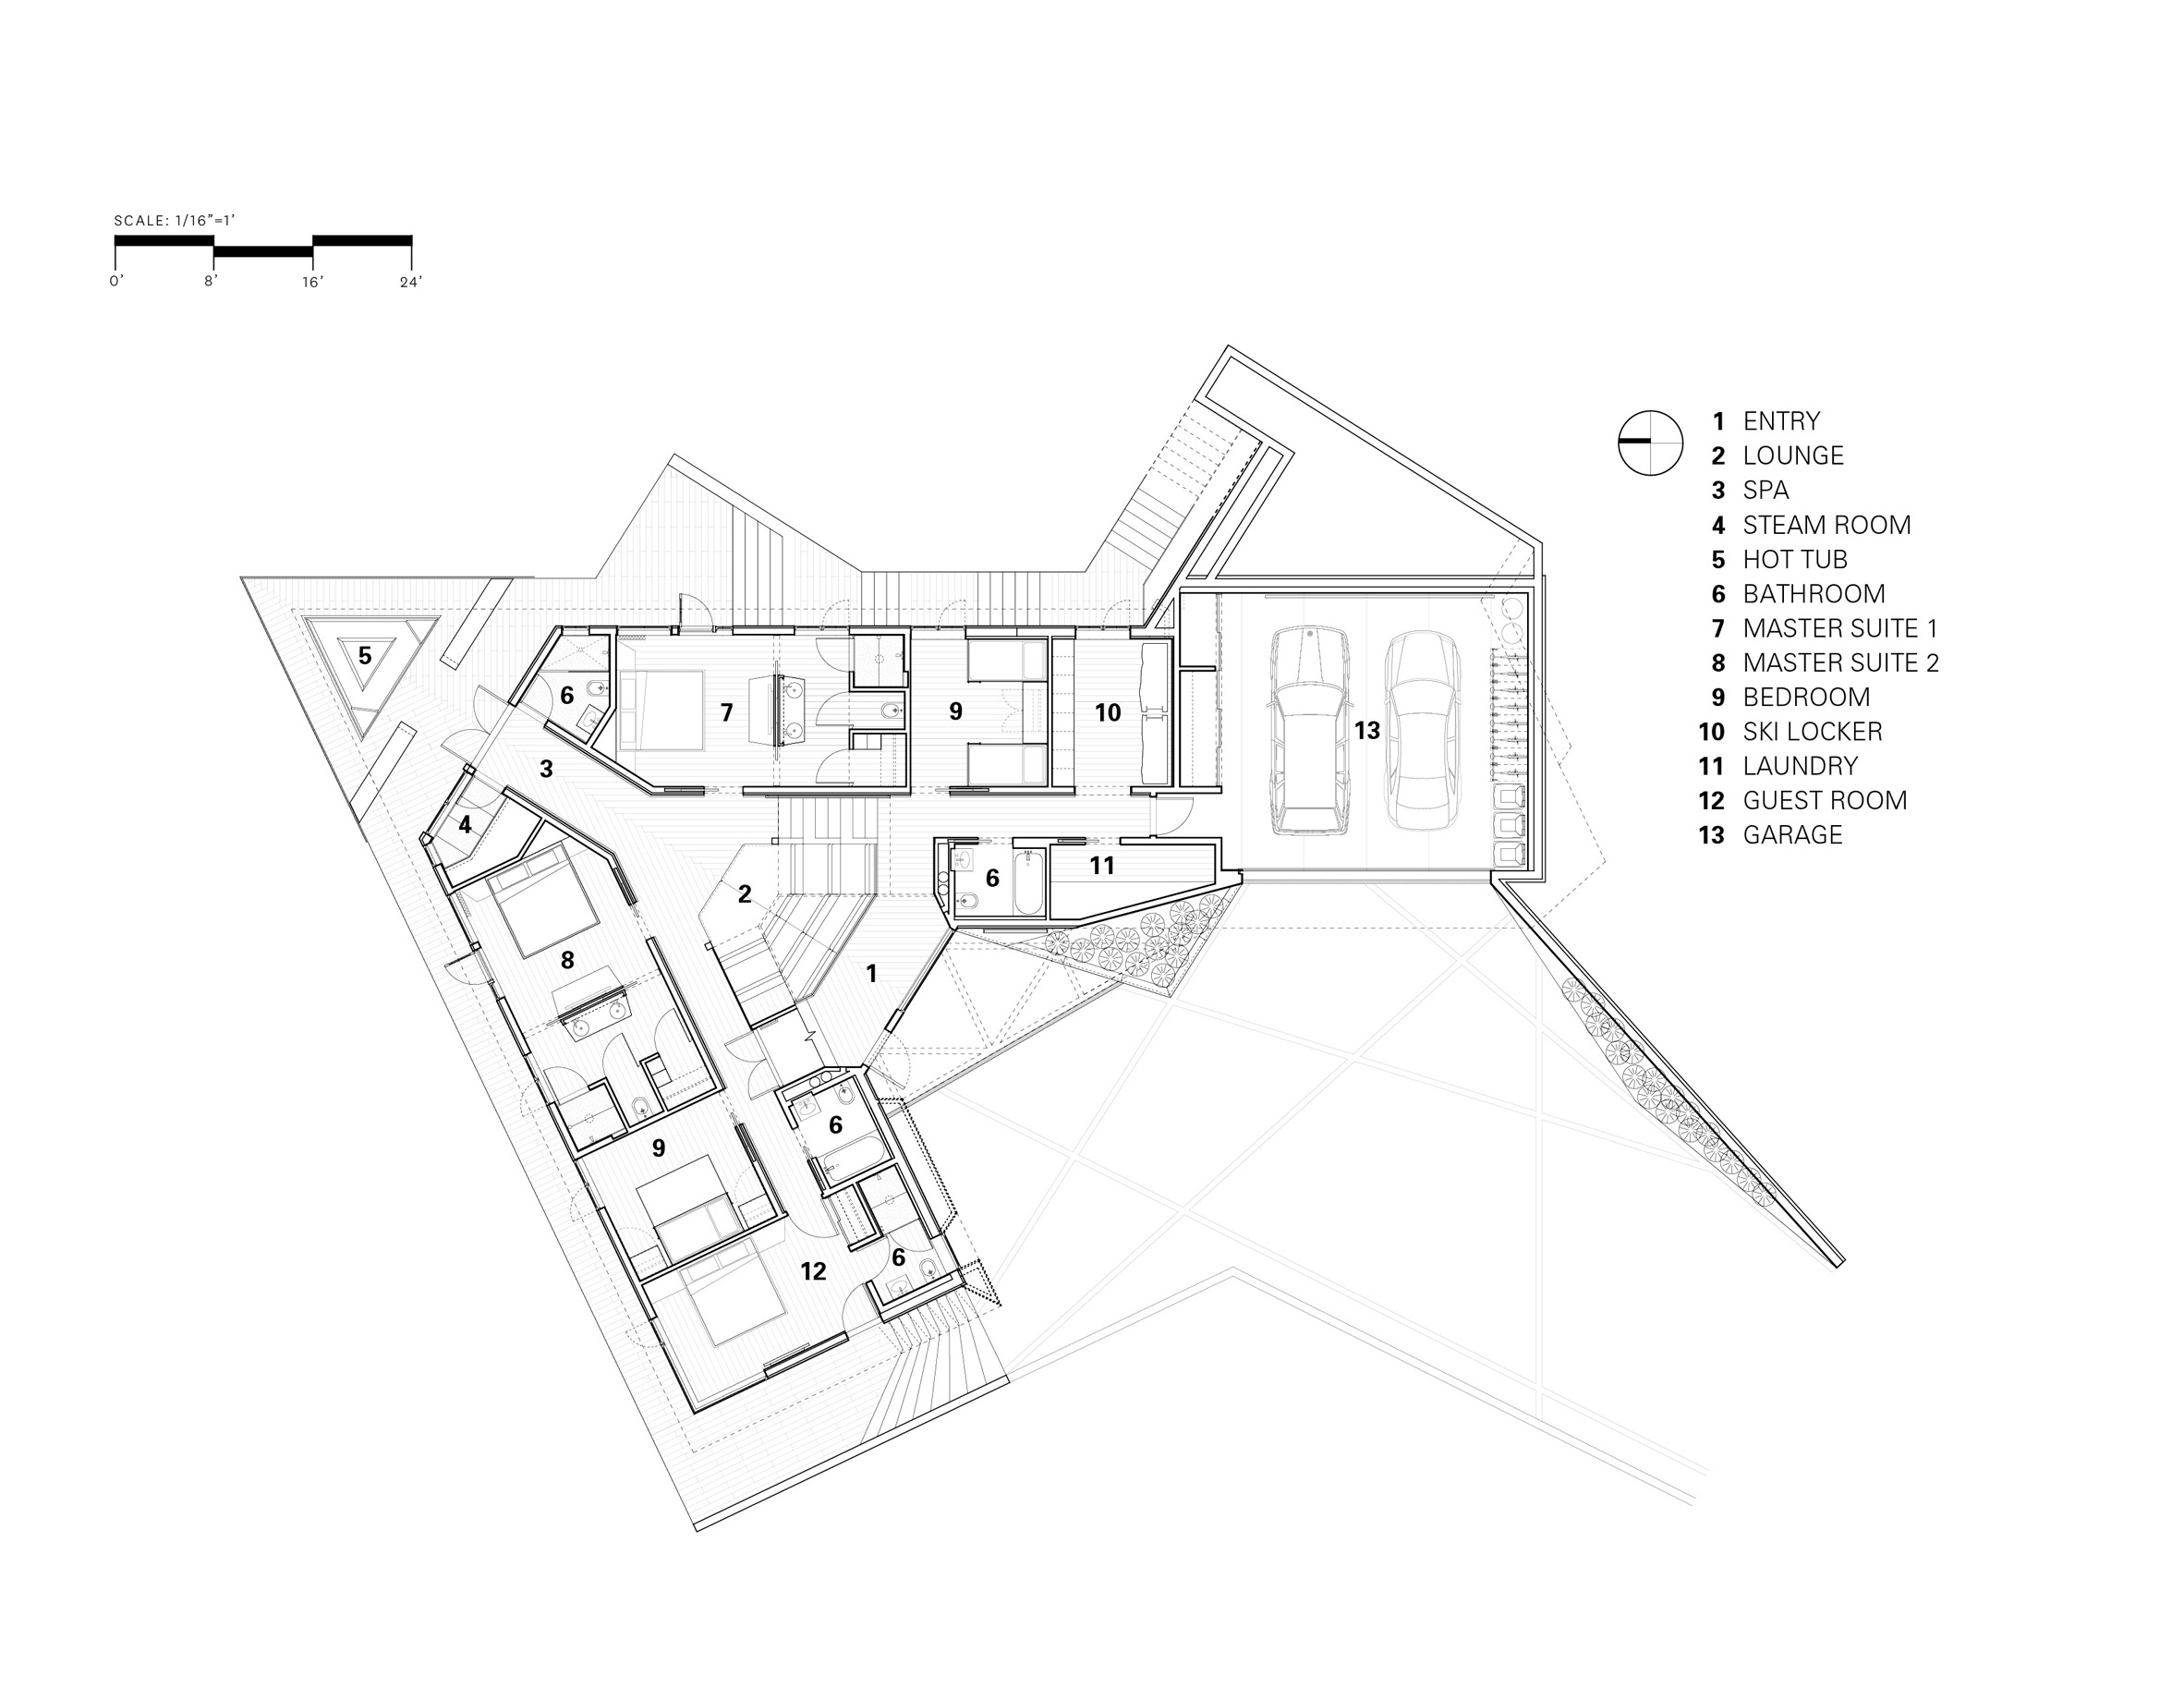
\includegraphics[width=1\textwidth]{fig/weird_floorplan.png}
    \label{}
    \caption[Weird floor plan]{Weird floor plan~\cite{weird_building}}
\end{figure}

When using a grid system apporach it will be possible to get an agent to walk from area 12 to 13 by specifically telling it which nodes are walkable and which nodes are not e.g walls. This will not be possible for the graph connectivity graph. The graph will here see only that area 12 and 13 are connected but not in which way. The method will draw a straight line between the two points and not see that the areas in reality are connected by the long pathway that goes through the entire floor plan.


\subsection{Grid system paper}
In this paper \cite{xu2017bim} they have the goal of solving “Accurate and efficient indoor path planning” in BIM models. The way they have implemented it is by using the grid system. 

\begin{figure}[H]
    \centering
    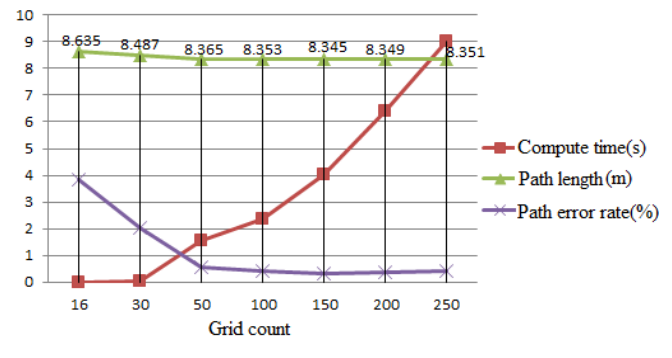
\includegraphics[width=1\textwidth]{fig/graph_grid_system.PNG}
    \caption{Graph showing computation cost as a function of grid count~\cite{xu2017bim}}
    \label{}
\end{figure}

They show what happens with the computation time when increasing the number of nodes. And also shows how minimal an effect it has on the path length.
%\section{Code notes}

\subsection{#1}
This is a function called dict_hashing. The purpose of this function is to hash the lines.

\subsection{Plotting rooms}
In this section we plot the floorplan outline and the rooms within it. We start by doing some simple preprocessing of the csv file with the rooms. 
The number of coordinates of each room is always dividable by 3 since it is created in such a way that each room is spanned by sets of triangles - hence it takes 3 coordinates to make up a triangle.

For each triangle we hash all lines in that triangle in a dictionary in both direction. This means that we hash 6 lines per triangle. The reason for this is that a triangle might have the same line as another triangle but in reverse order. These two lines should be seen as the same. Therefore we have to hash both directions of each line in every triangle.

For example say we have a line in one triangle (x1,y1) - (x2,y2). What we do is that we hash the line (x2,y2)-(x1,y1) as well. What happens now is that the other triangle has the same line but as (x2,y2) - (x1,y1). Just like the other triangle both directions will be hashed meaning (x1,y1)-(x2,y2). The way hashing works is that 2 identical values will give the same hash key. In this example we now have 2 values for 2 different hash keys, since the same line is occuring twice in 2 different hashes.

Now each dictionary element that has more than one value is removed. Therefore both of the hashes will be removed and we have made sure that the line is correctly removed.

Some other removal criterias are also present. This include manually removing lines/ walls that clearly are misplaced.

The way we hash also has the consequence of having each line existing twice in the dictionary. Therefore one of the directions of each line is removed. This makes the dictionary half as long and makes is more efficient for use later if need be.

At last we plot each line in the dictionary.
And repeat the process for a new room, setting the dictionary back to empty. The dictionary is concatenated with another dictionary that keeps all the lines of the floorplan for later use.


\subsection{Plotting the doors}
Again the program does some preprocessing on the csv file with the door coordinates. This csv file include the coordinate of each door and the direction it is facing. The last line of the csv consists of the coordinate translation.

For each door - depending on the direction it is facing - another door will be added on the other side of the wall it is facing. This makes it possible to go through doors. The reason for this will be explained in the TSP section.

Each door and its copy is then plotted.

\subsection{Adding room nodes}
The room nodes are the nodes are points of interest that the spot robot should visit. At this point the points are placed manually and arbitrarely. Later some algorithm will be made to place them.

\section{Traveling salesman approximate path}
\subsection{plotting all walkable paths}
The objective here is to for each node have which other nodes it can traverse to. The path between two nodes is not traversable if it is obstructed by a wall. 
An easy way to implement this is using a network datastructure. In this case the networkx framework is used. Nodes are created in the network for all points created - which includes door nodes and room nodes. 
Line intersection is them used to check if two nodes are traversable.
If they are traversable then we add an edge between the two nodes to the network with the weight of the edge being the euclidean distance between the two nodes.


\subsection{Shortest path between all "room" nodes}
The objective here is to find the shortest traversable path between all room nodes. This is usefull when we later want to find the minimum spanningtree and the approximate TSP solutions.

The networkx library has a function that performs dijkstras algorithm. A foor loop is run for each room node.The dijkstra function takes in the Network and a source node and outputs its distance to all other nodes and also the predecessors. The predecessors is for example if there are 4 nodes 1,2,3,4. If 1 and 4 is not directly connected, but are connected via node 2. What will happen is that the distance between 1 and 4 is still calculated in the distance output of the function but the predecessors for 2 will be 1 and for 4 will be 2 (if 1 is the source node).


\subsection{Make complete subgraph of all room nodes}
To use the approximate solutions of the tsp problem, many rely on the assumption of a complete graph. This means that all nodes in the graph are connected. One thing to note is that since we don't wish to find the tsp solution for all nodes (door,corner and room nodes) we wish to make a subgraph of only the room nodes. This graph should also be complete. 

This is done by first making a new graph that only include the room nodes.
We then compute the distance between each node in G_rooms using dijkstras function again.



\subsection{Minimum spanning tree}
This is a one line code that makes a minimum spanning tree given a network. This comes from the networkx framework. 
The minimum spanning tree is needed to do the approximate solution of the tsp problem.


\subsection{Solve TSP problem for subgraph using DFS traversal}
This is again a one line of code, where a depth first search traversal is performed on the minimum spanning tree of the rooms. 

The next step to finalize the tsp solution is to remove double vertices occuring when doing the depth first seach algorithm on the minimum spanning tree.

The dfs list consists of node pairs with a 'from' node and a 'to' node.
e.g
(1,2), (2,3), (3,4) etc.
We can have that the 'from' node of the current node pair is not the 'to' node of the previous node pair. 
e.g
(1,2), (1,3)
When this happens we want to make i a shortcut such that it goes directly from 2 to 3 without going back to one.


We do this by having a for loop that runs through all node pairs in the list of the depth first search edges. 
If the 'to' node in the previous node pair
is not the same as the from node in the next node pair then the new 'from' node should be the previous 'to' node and the new 'to' node
should be the current 'to' node.
For example if we have (1,2), (1,3) then because we go back to 1 we change it to (1,2), (2,3).



\subsection{#9}
\subsection{#10}
%\section{Noter}
\subsection{Noter til Paper}
Trying to solve “Accurate and efficient indoor path planning” since a lot of people uses indoor walking. There are challenges with indoor navigation.
\\\\
Industry Foundation Classes (IFC)
Semantic information in BIM models
Revit
Triangular prism subdivision
Geometric and semantic information
2D grid subdivision and 3D space subdivision based on triangular prism.
How about if you use variable sizes of grid, depending on the rooms.


\subsection{Noter til master these:Pathfinding in Two-dimensional
Worlds }

You can represent the 2D world in 2 ways, as a 8-grid system and a polygonal way. The problems with the grid system are suboptimal path length and the problem of choosing a fitting grid resolution.

Polygons works by connecting each portruding corner and making a connection graph.

A* works on graphs and grids
JPS (jump point search) works on grids only, and is good for large areas of open space.

HPA is also a good algorithm for grid systems but is not necessarily optimal. At most 1\% worse than optimal. Makes use of preprocessing, and clusters the map and makes a graph of higher abstractions such that it gets an overview of the overall structure of the map before doing the pathfinding.
A fitting cluster size is also of importance for HPA* as we saw in the Scaled Maze map.

VG (visibility graph)
is an algorithm that works on polygonal maps.



\subsection{Noter process og generelle tanker}
\subsubsection{Rapport tanker}
Rapporten består af undersøgende arbejde og er vigtigere end implementationen.
Rapport bliver vurderet på diskussion.
Man kan gøre det på mange måder.
Ulempen ved connectivitet er at man ikke kan se væggene. Graph måden.
Find så mange metoder som muligt og skriv hvorfor de andre er dårlige. 
Det viser at du har tænkt dig. 
Rapport stuff: for og imod forskellige implementationer.
Kriterie liste med fordele og ulemper.
Undersøg begge veje, og argumenter.
Undersøg på papir og læs dig frem til det. Skriv for og imod for begge. 
Læs en masse artikler, og skriv alle tanker omkring det.

\subsubsection{Ugentlige rapporter}
Hvad skete I den forgangne uge, hvad har været nogle problemer.
Ugerapport der beskriver status.
Skriv nogle noter til jer selv.
Små tekst stumper
Trello planlægning, to do liste
Include figures and bibtex and notes.


\subsubsection{Brainstorm}
Lav en meget præcis liste med ting du skal have gjort så du altid har noget at lave.
Brug en time på det i to doist.

Hvad skal jeg gøre i sidste ende?
Robotten skal kunne bevæge sig fra punkt til punkt i en bygning mens den tager billeder på en etage. Den skal have en strategi til hvordan den går rundt og hvordan den undviger forhindringer.

En meget overordnet planlægning af hvordan du kommer systematisk rundt i en bygning, så den kan blive scannet.
Denne opgave behøver ikke være så geometrisk. Du kan egentlig se en bygning som en graf, hvor hver knude svarer til et rum.

Det andet element er at komme rundt i de enkelte rum og gå fra rum til rum på en hensigtsmæssig måde.
How to compare different methods?


% \input{References.bib}
%\tableofcontents
%\thispagestyle{empty}
%\newpage
%\printbibliography
% \bibliographystyle{plain}
% \bibliography{References.bib}
% \newpage
\printbibliography
\end{document}

   